Assurance of data integrity has been one of the most fundamental aspects of hardware, software, and network protocols.
Different mechanisms of error tolerance, detection, and mitigation have been widely implemented and deployed in different layers of 
the compute, storage, network, and applications systems.

However, due to the insufficient capability of existing protocols, incomplete end-to-end data integrity coverage, 
and more possible component bugs in highly distributed and complex systems, integrity errors can become undetected in 
the system, dubbed {\it `silent errors'}.  Unaccountable integrity errors not only degrade the application performance, but also pass the corrupted data
to the critical applications that may lead to catastrophic results~\cite{Jung2019HighPerformanceEI}.

Certain bugs in CPUs, switches, and software can cause data integrity errors that would evade the existing error capture mechanisms.
For example, Facebook recently reported a CPU bug that caused severe silent data corruption in its hyper-scale data 
centers~\cite{facebook:cpu:2021}. A bug in a network switch that caused random data corruption and bypassed the TCP checksum 
mechanism was also reported in a production network~\cite{swip:pearc:2019}. It is well known that the Ethernet CRC and TCP checksums are 
too small for modern data sizes~\cite{tcp:ccr2000}.

While the probability of undetected integrity errors seems to be extremely low, the proliferation of big data accompanied by the ever-growing scales of Internet, 
Cloud, IoT (Internet of Things), and HPC (High-Performance Computer) in recent years has amplified the challenges to maintain high data integrity for 
Internet applications that often rely on distributed compute and storage systems over wide-area networks. For example, it was estimated that up to 1 in 10 billion 
TCP segments may encounter undetected TCP checksum error in~\cite{tcp:ccr2000}. A simple calculation tells that 10 billion maximum Ethernet frames translates to 
only 3.4 hours of data transfer on a 10gbps (gigabit per second) link. 

The traditional redundancy measures of retransmission and various fault tolerance mechanisms are designed to mask the negative impacts of the errors.
However, the emerging systems of large scale and exponentially growing data volumes have made these measures less efficient and prohibitively expensive to deploy 
widely~\cite{GrayFailure:2017}.

These recent development has led to renewed interests in integrity error detection and mitigation techniques at the end-to-end file transfer level. 
Several prominent Internet application softwares have added such integrity error checksum capability in an attempt to prevent the data corruptions 
from getting to their final user  applications~\cite{IntegrityVerification:DataTransfer}. While the application systems can help with the detection of the silent errors, t
he ultimate solution is to identify the root causes so that the right culprit(s) in the system, be it the faulty hardware components or operational factors, can be promptly localized, replaced or reconfigured. 

In general, localizing any kinds of failures in the complex distributed Internet system remains a difficult task which has been done mostly through manual debugging. 
It is well understood that the main barriers come from the exponentially growing scale of the system and the reality that the 
infrastructure system is divided and conquered by different administrative parties in multiple network domains, storage and compute subsystems in data centers at different sites. 
Vertically, there are different middleware and applications running end-to-end on top of the infrastructural system. These two barriers implies several realistic constraints 
in automating the debugging process with software: lack of comprehensive monitoring capabilities, less likelihood in freely sharing system and real-time monitoring information across 
the horizontal and vertical boundaries, daunting job to process huge volume of monitoring data, 


 the intermittent and random nature of 
the distributed nature and stringent resources of WSNs render it hard for a network operator to completely monitor the system?s working status.
On the other hand, the interactions within the WSN and the causal dependencies between root causes and symptoms are usually unknown.
As a result, silent failures remain undetected.

It belongs to the broader {\it'gray failures'}, {\it'silent failures'}, {\it'probabilistic failures'}  in contrast to the {\it fail-stop} failures where

damages: service disruption, waste of time in retrying, data corruption leading to wrong results and decisions. 
  
Error tolerance, redundancy, overhead in resource and latency

end-too-end check at the file or block level, overhead in computing and latency.

localization has been ignored

error family and error locations at different granularity 




It has been recently recognized that existing protection mechanisms commonly implemented in Internet and distributed systems such as TCP checksums and redundant coding in storage systems are not sufficient to handle silent {\it gray failures}, which often lead to wide spread system slowdown, application malfunction, and corrupted data. As a result, advanced distributed systems started to add extra end-to-end data integrity checks to catch these failures early on in order to reduce application failures and blind retries~\cite{swip:pearc:2019}. 

However, identifying the root causes of these gray failures remains a largely unsolved problem due to the challenges presented in Section~\ref{sec:introduction}: 
incomplete network state information, intermittent probabilistic nature of gray failures, and complexity in diagnosing complex networks in a scalable fashion.  

A network system can be modeled as a graph with a set of nodes connected by links via interfaces. The nodes in the network consist of end hosts (that generate and receive data) and networking devices (routers or switches). Due to scalability or privacy constraints, deploying monitoring capabilities at every point of the targeted large-scale network is not possible. Therefore, the problem can be concisely modeled as a bipartite mapping graph between the path level flows and its network components as shown in Fig.~\ref{fig:bipartite}. What makes the problem extremely difficult is that the mapping relationships in the bipartite graph are unknown. We further observe that one component failure (e.g., $L_j$) will cause multiple paths erroneous while one flow error (e.g., $F_i$) may be caused by multiple component failures. And because the component gray failure probability is normally low ($10^{-3} - 10^{-6}$), it would require large number of file transfers to catch a few number of corrupted files. Our ultimate goal is to localize the possible root causes in node or link errors by inference from the observed flow level abnormalities only at the end hosts, which can be translated to learning the mappings in such a graph.

\begin{wrapfigure}{ht}{0.25\textwidth}
  \begin{center}
    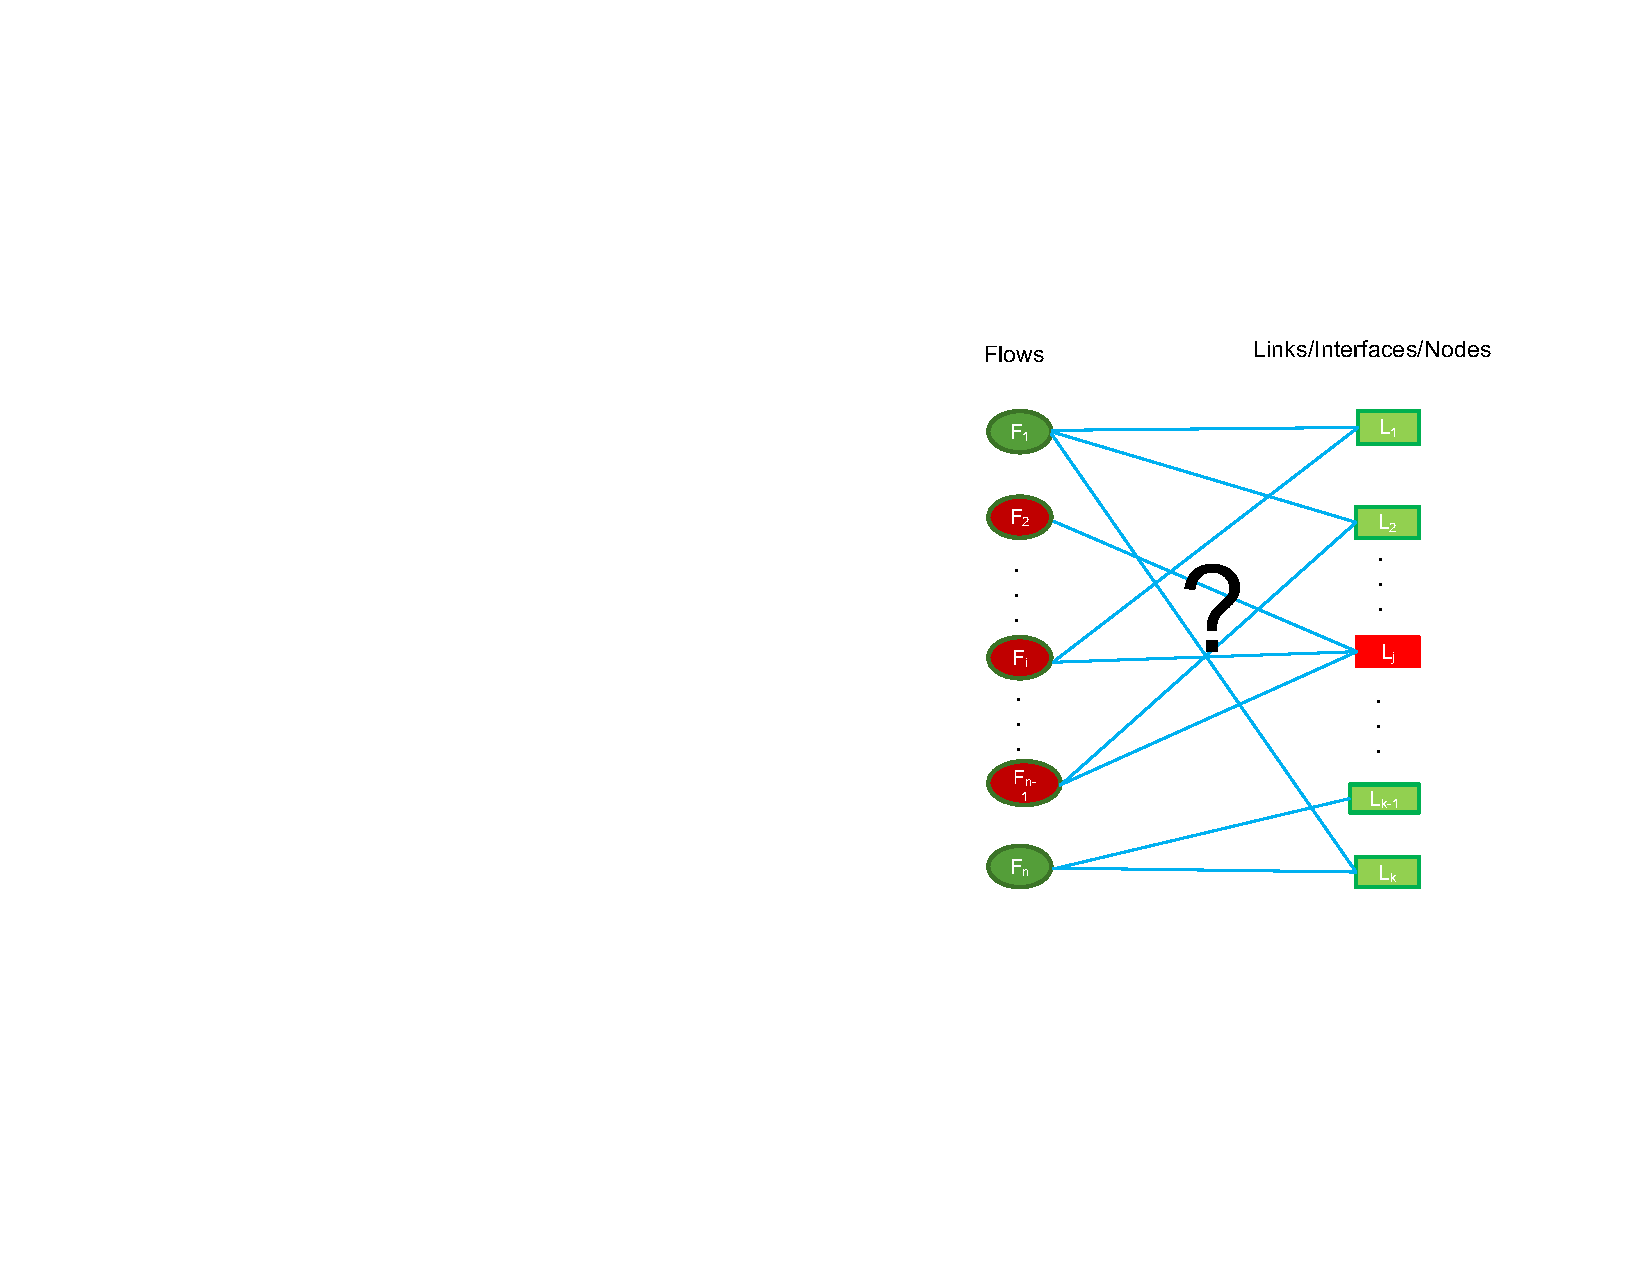
\includegraphics[width=0.25\textwidth]{./figure/RCABipartite}
  \end{center}
  \vspace{-5pt}
\caption{RCA Bipartite Graph}
\vspace{-5pt}
\label{fig:bipartite}
\end{wrapfigure}

The majority of recent work assume flow information between any pair of nodes in the network is available because they focus on data center networks that they have full ownership and modern routers allow originating and receiving probing data. This is very important because, as shown in~\cite{netbouncer:nsdi18}, there exists a minimal set of source-destination pairs to guarantee successful pinpointing of link errors in the network. Some of the work further assume they even know the routes for every flow, i.e., the mapping represented in Fig.~\ref{fig:bipartite}. However, both assumptions do not hold for our targeted multi-domain network environment due to obvious administrative constraints and the fact that, in the Internet scale network, traffic routing and forwarding are largely dynamically decided by the control plane software like OSPF and BGP subject to frequent topology and policy changes. 

We therefore made more restrictive but more realistic assumptions in this study in that (1) only the data file transfer information including integrity error states can be obtained at the end hosts from application layer; (2) only the physical nodes (domains) and their interfaces are known to us, but the network topology and traffic routing are unknown. 

In a large network, collecting the passive monitoring data from all node pairs may not scale well. Therefore, injecting probe packets between the designated node pairs periodically is adapted by several existing RCA systems. In practice, due to the probabilistic nature of the grey failures, controlled fault injection is an efficient way to generate training data within a reasonable time frame.

Directly accessing the production system to instrument the analysis with either active probing or fault injection is not realistic in most cases, especially in a multi-domain system where no one owns the entire infrastructure like in the data center networks. We believe emulation with realistic scales is a viable choice, given advanced Cloud testbeds are available.








